\documentclass{beamer}\usepackage[]{graphicx}\usepackage[]{color}
%% maxwidth is the original width if it is less than linewidth
%% otherwise use linewidth (to make sure the graphics do not exceed the margin)
\makeatletter
\def\maxwidth{ %
  \ifdim\Gin@nat@width>\linewidth
    \linewidth
  \else
    \Gin@nat@width
  \fi
}
\makeatother

\definecolor{fgcolor}{rgb}{1, 0.894, 0.769}
\newcommand{\hlnum}[1]{\textcolor[rgb]{0.824,0.412,0.118}{#1}}%
\newcommand{\hlstr}[1]{\textcolor[rgb]{1,0.894,0.71}{#1}}%
\newcommand{\hlcom}[1]{\textcolor[rgb]{0.824,0.706,0.549}{#1}}%
\newcommand{\hlopt}[1]{\textcolor[rgb]{1,0.894,0.769}{#1}}%
\newcommand{\hlstd}[1]{\textcolor[rgb]{1,0.894,0.769}{#1}}%
\newcommand{\hlkwa}[1]{\textcolor[rgb]{0.941,0.902,0.549}{#1}}%
\newcommand{\hlkwb}[1]{\textcolor[rgb]{0.804,0.776,0.451}{#1}}%
\newcommand{\hlkwc}[1]{\textcolor[rgb]{0.78,0.941,0.545}{#1}}%
\newcommand{\hlkwd}[1]{\textcolor[rgb]{1,0.78,0.769}{#1}}%
\let\hlipl\hlkwb

\usepackage{framed}
\makeatletter
\newenvironment{kframe}{%
 \def\at@end@of@kframe{}%
 \ifinner\ifhmode%
  \def\at@end@of@kframe{\end{minipage}}%
  \begin{minipage}{\columnwidth}%
 \fi\fi%
 \def\FrameCommand##1{\hskip\@totalleftmargin \hskip-\fboxsep
 \colorbox{shadecolor}{##1}\hskip-\fboxsep
     % There is no \\@totalrightmargin, so:
     \hskip-\linewidth \hskip-\@totalleftmargin \hskip\columnwidth}%
 \MakeFramed {\advance\hsize-\width
   \@totalleftmargin\z@ \linewidth\hsize
   \@setminipage}}%
 {\par\unskip\endMakeFramed%
 \at@end@of@kframe}
\makeatother

\definecolor{shadecolor}{rgb}{.97, .97, .97}
\definecolor{messagecolor}{rgb}{0, 0, 0}
\definecolor{warningcolor}{rgb}{1, 0, 1}
\definecolor{errorcolor}{rgb}{1, 0, 0}
\newenvironment{knitrout}{}{} % an empty environment to be redefined in TeX

\usepackage{alltt}
\usepackage{../371g-slides}
% Uncomment these lines to print notes pages
% \pgfpagesuselayout{4 on 1}[letterpaper,border shrink=5mm,landscape]
% \setbeameroption{show only notes}
\title{Probability review 2}
\subtitle{Lecture 4}
\author{STA 371G}
\IfFileExists{upquote.sty}{\usepackage{upquote}}{}
\begin{document}



\frame{\maketitle}
\begin{darkframes}

\begin{frame}{Reading assignments}
  \begin{itemize}[<+->]
    \item Reading assignments help you build (incomplete) mental structures that we can build on in class
    \item Your assignment is to read and annotate: ask a question, answer a classmate's question, make an observation, try to explain something better than the text does
    \item Make at least three high-quality annotations per document to get full credit (examples on Canvas)
    \item Each assignment is graded on a 0-3 scale; you'll get full credit for a 2
    \item First assignment is due \textbf{Sunday, February 4 at 7:00 PM}
    \item See handout on Canvas (under Files) for more information and examples
  \end{itemize}
\end{frame}


\begin{frame}
  \fullpagepicture{muppets.jpg}
\end{frame}

\begin{frame}{Who are these guys?}
  \begin{columns}[onlytextwidth]
    \column{.25\textwidth}
      \begin{center}
        
\includegraphics[width=1in]{kermitthefrog} \\
      \end{center}
    \column{.25\textwidth}
      \begin{center}
        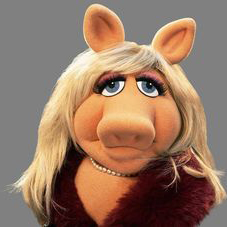
\includegraphics[width=1in]{misspiggy} \\
      \end{center}
    \column{.25\textwidth}
      \begin{center}
        
\includegraphics[width=1in]{swedishchef} \\
      \end{center}
    \column{.25\textwidth}
      \begin{center}
        
\includegraphics[width=1in]{rowlf} \\
      \end{center}
  \end{columns}
  \smallskip
  \begin{columns}[onlytextwidth]
    \column{.3\textwidth}
      \begin{center}
        
\includegraphics[width=1in]{statler} \\
      \end{center}
    \column{.3\textwidth}
      \begin{center}
        
\includegraphics[width=1in]{waldorf} \\
      \end{center}
    \column{.3\textwidth}
      \begin{center}
        
\includegraphics[width=1in]{fozziebear} \\
      \end{center}
  \end{columns}
\end{frame}

\begin{frame}{Who are these guys?}
  \begin{columns}[onlytextwidth]
    \column{.25\textwidth}
      \begin{center}
        
\includegraphics[width=1in]{kermitthefrog} \\
        Kermit the Frog
      \end{center}
    \column{.25\textwidth}
      \begin{center}
        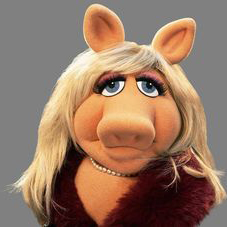
\includegraphics[width=1in]{misspiggy} \\
        Miss Piggy
      \end{center}
    \column{.25\textwidth}
      \begin{center}
        
\includegraphics[width=1in]{swedishchef} \\
        Swedish Chef
      \end{center}
    \column{.25\textwidth}
      \begin{center}
        
\includegraphics[width=1in]{rowlf} \\
        Rowlf the Dog
      \end{center}
  \end{columns}
  \smallskip
  \begin{columns}[onlytextwidth]
    \column{.3\textwidth}
      \begin{center}
        
\includegraphics[width=1in]{statler} \\
        Statler
      \end{center}
    \column{.3\textwidth}
      \begin{center}
        
\includegraphics[width=1in]{waldorf} \\
        Waldorf
      \end{center}
    \column{.3\textwidth}
      \begin{center}
        
\includegraphics[width=1in]{fozziebear} \\
        Fozzie Bear
      \end{center}
  \end{columns}
\end{frame}

\begin{frame}
  \begin{columns}[onlytextwidth]
    \column{.2\textwidth}
      
\includegraphics[width=0.45in]{kermitthefrog} \\
      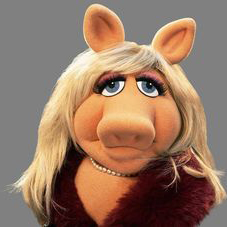
\includegraphics[width=0.45in]{misspiggy} \\
      
\includegraphics[width=0.45in]{swedishchef} \\
      
\includegraphics[width=0.45in]{rowlf} \\
      
\includegraphics[width=0.45in]{statler} \\
      
\includegraphics[width=0.45in]{waldorf} \\
      
\includegraphics[width=0.45in]{fozziebear} \\
    \column{.8\textwidth}
      Suppose we pick a Muppet at random. Each of these are events:
      \begin{itemize}[<+->]
        \item $A = $ we select an animal (non-human?)
        \item $B = $ we select someone who is bald
      \end{itemize}
      \pause
      $P(A) = \pause 4/7$ \qquad $P(B) = \pause 3/7$
  \end{columns}
\end{frame}

\begin{frame}
  \begin{columns}[onlytextwidth]
    \column{.2\textwidth}
      
\includegraphics[width=0.45in]{kermitthefrog} \\
      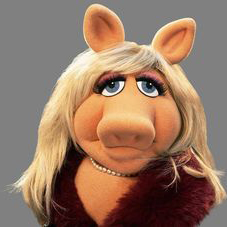
\includegraphics[width=0.45in]{misspiggy} \\
      
\includegraphics[width=0.45in]{swedishchef} \\
      
\includegraphics[width=0.45in]{rowlf} \\
      
\includegraphics[width=0.45in]{statler} \\
      
\includegraphics[width=0.45in]{waldorf} \\
      
\includegraphics[width=0.45in]{fozziebear} \\
  \column{.8\textwidth}
    \begin{itemize}
      \item $A|B = $ we select at random from among the bald characters, and get an animal
      \item $B|A = $ we select at random from among the animals, and get a bald Muppet
    \end{itemize}
    \[
      P(A) = 4/7 \qquad P(B) = 3/7
    \]
    \pause
    \begin{align*}
      P(A|B) &= \frac{\text{\# bald animals}}{\text{\# bald Muppets}} = \frac{P(\text{$A$ and $B$})}{P(B)} = \frac 1 3 \\
      P(B|A) &= \frac{\text{\# animals}}{\text{\# animal Muppets}} = \frac{P(\text{$A$ and $B$})}{P(A)} = \frac 1 4 \\
    \end{align*}
  \end{columns}
\end{frame}

\begin{frame}
  \begin{columns}[onlytextwidth]
    \column{.2\textwidth}
      
\includegraphics[width=0.45in]{kermitthefrog} \\
      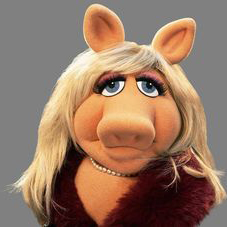
\includegraphics[width=0.45in]{misspiggy} \\
      
\includegraphics[width=0.45in]{swedishchef} \\
      
\includegraphics[width=0.45in]{rowlf} \\
      
\includegraphics[width=0.45in]{statler} \\
      
\includegraphics[width=0.45in]{waldorf} \\
      
\includegraphics[width=0.45in]{fozziebear} \\
  \column{.8\textwidth}
    \begin{itemize}
      \item $A|B = $ we select at random from among the bald characters, and get an animal
      \item $B|A = $ we select at random from among the animals, and get a bald character
    \end{itemize}
    \begin{align*}
      \onslide<1->{P(\text{$A$ and $B$}) &= P(\text{select bald animal from all Muppets}) \\}
      \onslide<2->{ &= 1/7 \\}
      \onslide<3->{ &= P(A)P(B|A) = \frac 4 7 \cdot \frac 1 4 \\}
      \onslide<3->{ &= P(B)P(A|B) = \frac 3 7 \cdot \frac 1 3 \\}
      \onslide<4->{ &\neq P(A)P(B)}
    \end{align*}
  \end{columns}
\end{frame}

\begin{frame}
  \begin{columns}[onlytextwidth]
    \column{.2\textwidth}
      
\includegraphics[width=0.45in]{kermitthefrog} \\
      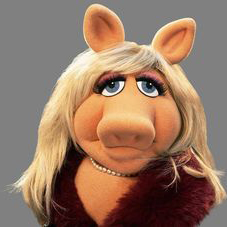
\includegraphics[width=0.45in]{misspiggy} \\
      
\includegraphics[width=0.45in]{swedishchef} \\
      
\includegraphics[width=0.45in]{rowlf} \\
      
\includegraphics[width=0.45in]{statler} \\
      
\includegraphics[width=0.45in]{waldorf} \\
      
\includegraphics[width=0.45in]{fozziebear} \\
  \column{.8\textwidth}
    The easy multiplication rule $P(\text{$A$ and $B$})=P(A)P(B)$ does not work because baldness and animalness are \emph{not} independent!
    \pause
    \begin{itemize}[<+->]
      \item If a Muppet is bald, they are less likely to be an animal
      \item If a Muppet is an animal, they less likely to be bald
    \end{itemize}
    \pause
    The more complex rule $P(\text{$A$ and $B$})=P(A)P(B|A)$ will always work.
  \end{columns}
\end{frame}


\begin{frame}
  \begin{columns}[onlytextwidth]
    \column{.2\textwidth}
      
\includegraphics[width=0.45in]{kermitthefrog} \\
      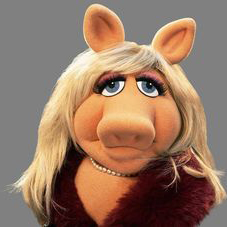
\includegraphics[width=0.45in]{misspiggy} \\
      
\includegraphics[width=0.45in]{swedishchef} \\
      
\includegraphics[width=0.45in]{rowlf} \\
      
\includegraphics[width=0.45in]{statler} \\
      
\includegraphics[width=0.45in]{waldorf} \\
      
\includegraphics[width=0.45in]{fozziebear} \\
    \column{.8\textwidth}
      \begin{align*}
        \onslide<1->{P(\text{$A$ or $B$}) &= \text{probability of selecting an animal,} \\ & \qquad\text{a bald Muppet, or both}\\}
        \onslide<2->{ &= 6/7 \\}
        \onslide<3->{ &= P(A) + P(B) - P(\text{$A$ and $B$}) \\ &= 4/7 + 3/7 - 1/7 \\}
      \end{align*}
      \pause\pause\pause
      We have to subtract off $P(\text{$A$ and $B$})$ because otherwise we are double-counting Kermit! (Poor Kermit: it's not easy being green.)
  \end{columns}
  \note{Do LC questions 2-6 after this slide.}
\end{frame}


\begin{frame}{Conditional probability}
  \begin{center}
    When we say $P(A|B)$, what we mean is:
    \bigskip

    ``In a world where we know B has already happened, how likely is it that A also happened?''
  \end{center}
\end{frame}

\begin{frame}
  \note{Imagine you are living with a partner---your husband/wife/boyfriend/girlfriend---and you come home one day to find underwear of unknown origin on your bedroom dresser!}
  \fullpagepicture{dresser}
\end{frame}

\begin{frame}
  \note{What do you do---besides this?!}
  \fullpagepicture{reaction}
\end{frame}

\begin{frame}
  \begin{center}
    Now that you’ve found a strange pair of underwear in your dresser, what is the probability that your partner is cheating on you?
    \bigskip
    \[ P(\text{partner is cheating} \mid \text{underwear found}) \]
    \pause\bigskip
    It's hard to know how to estimate this directly!
  \end{center}
\end{frame}

\begin{frame}
  Let's come up with estimates for the following:
  \begin{itemize}[<+->]
    \item $P(\text{underwear found} \mid \text{partner is cheating}) = P(U|C)$
    \item $P(\text{underwear found} \mid \text{partner is not cheating}) = P(U|\overline C)$
    \item $P(\text{partner is cheating}) = P(C)$ (before we found the underwear!)
  \end{itemize}
  Now that we found the underwear, we want to \emph{update our estimate} of how likely it is that our partner is cheating, i.e., we want to know $P(C|U)$.
  \newline\pause
  (Note: This is the \emph{reverse} of the probability we know already!)
\end{frame}

\begin{frame}{Let's figure it out!}
  \note{Let students do the calculations using the estimates students \textCR
  came up with in the previous slide. Use the LC questions to gather responses.}

  Since $P(\text{$C$ and $U$}) = P(C|U)P(U)$,

  \[ P(C|U) = \frac{P(\text{$C$ and $U$})}{P(U)}. \]

  \pause

  Now we just need to figure out $P(\text{$C$ and $U$})$ and $P(U)$!
\end{frame}

\begin{frame}{Let's figure it out!}
  There are two mutually-exclusive ways you could find underwear in the drawer: if your partner is cheating, and if they aren't cheating. \pause  So:
  \[
    P(U) = P(\text{$U$ and $C$}) + P(\text{$U$ and $\overline{C}$})
  \]
\end{frame}

\end{darkframes}
\end{document}
